% UTF-8

% single-chapter commands
\documentclass[../main/thesis.tex]{subfiles}
\onlyinsubfile{\appendix}  % single-chapter command
\begin{document}



\chapter{Mathematische Konventionen}
\label{appx:mathsymbols}
% zu 4

{\setlength{\doublerulesep}{1mm}%\renewcommand{\arraystretch}{1.1}
\begin{longtable}[c]{|c|p{12cm}|}
\hline
\textbf{Symbol} & \textbf{Beschreibung} \\
\hline
\hline
\endhead
\caption*{(fortgesetzt)}
\endfoot
\caption{Mathematische Abkürzungen und Symbole}
%\label{tab:mathsymbols}
\endlastfoot
\multicolumn{2}{|l|}{\textbf{Bezeichner}} \\
\hline
$\alpha,\beta,\gamma,...$ & Griechische Kleinbuchstaben bezeichnen reelle Größen mit oder ohne Dimension wie Winkel, Längen oder Verhältniszahlen. \\
\hline
$a,b,c,...$ & Lateinische Kleinbuchstaben bezeichnen in aller Regel Vektoren. \newline Lediglich solche reelle Größen, für die ein lateinischer Buchstabe im jeweiligen Kontext fest etabliert ist, werden mit lateinischen Buchstaben bezeichnet. \\
\hline
$A,B,C,...$ & Lateinische Großbuchstaben bezeichnen Mengen. \\
\hline
\hline
\multicolumn{2}{|l|}{\textbf{Arithmetik}} \\
\hline
$\abs[\alpha]$ & absoluter Betrag der Zahl $\alpha$ \\
\hline
$\abs[a]$ & geometrische Länge des Vektors $a$ \\
\hline
$\sphericalangle(a,b)$ & gerichteter rechtsdrehender Winkel von $a$ zu $b$ im Intervall $(-\pi,\pi)$ \\
\hline
\hline
\multicolumn{2}{|l|}{\textbf{Logische Aussagen}} \\
\hline
$\wedge$ & und \\
\hline
$\forall\, M$ & für alle Elemente der Menge $M$ \\
\hline
$\exists\ a$ & es existiert ein $a$ \\
\hline
$:$ & so dass gilt \\
\hline
\hline
\multicolumn{2}{|l|}{\textbf{Mengen}} \\
\hline
\multicolumn{2}{|p{13cm}|}{Mengen sind ungeordnet und können kein Element mehrfach enthalten.} \\
\hline
$\set{a,b}$ & Menge bestehend aus den Elementen $a$ und $b$ \\
\hline
$\TheEmptySet$ & leere Menge \\
\hline
$\abs M \abs$ & Anzahl der Elemente der Menge \\
\hline
$\cup$ & Vereinigung \hfill $\set{a,b} \cup \set{b,c} = \set{a,b,c}$ \\
\hline
$\cap$ & Schnittmenge \hfill $\set{a,b} \cap \set{b,c} = \set{b}$ \\
\hline
$\setminus$ & Restmenge (gelesen „ohne“) \hfill $\set{a,b} \setminus \set{b,c} = \set{a}$ \\
\hline
$\in$ & Element in Menge \hfill $a \in \set{a,b}$ \\
\hline
$\subset$ & Teilmenge \hfill $\set{a} \subset \set{a,b}$ \\
\hline
\hline
\multicolumn{2}{|l|}{\textbf{Algorithmen}} \\
\hline
$\textproc{Name}$ & Kurzbezeichnung eines Algorithmus durch dessen Namen \\
\hline
$\equiv$ & identisch mit \newline (es folgt die Definition des linksseitigen Bezeichners, z.~B. durch eine Abfolge von Arbeitsschritten) \\
\hline
$\triangleright$ & Kommentar \\
\hline
$\gets$ & Zuweisung \\
\hline
\algorithmicforall & wiederhole die folgenden eingerückten Schritte nacheinander einmal für jedes Element der angegebenen Menge \\
\hline
\algorithmicwhile & wiederhole die folgenden eingerückten Schritte nacheinander solange, wie die angegebene Bedingung wahr ist \\
\hline
\algorithmicif & führe die folgenden eingerückten Schritte nur aus genau dann, wenn die angegebene Bedingung wahr ist \\
\hline
\textbf{Ergebnis} & Ergebnis des Algorithmus (Rückgabewert) \\
\hline
$\rightarrow$ & Definition einer Relation (Assoziation) der genannten Datentypen \\
\hline
{\small$\eqdef$} & Definition des Anfangswerts einer Relation \\
\hline
$\mathcal{O}(f)$ & Menge aller Algorithmen, deren Rechenaufwand nicht wesentlich schneller als $f$ wächst \\
\hline
$\hbox{o}(f)$ & Menge aller Algorithmen, deren Rechenaufwand wesentlich langsamer als $f$ wächst \\
\hline
\hline
\multicolumn{2}{|l|}{\textbf{Einheiten und Datentypen}} \\
\hline
px & Pixel \newline die kleinste rechteckige Fläche in gerasterter Darstellung, z.~B. auf dem Bildschirm (für \osm\ in der Regel quadratisch); \newline als Längeneinheit: die Länge einer Pixelreihe von 1\,px Breite \\
\hline
boolean & wahr oder falsch (bezogen auf logische Aussagen) \\
\hline
\end{longtable}
}



\chapter{Bezeichner im Quelltext}
\label{appx:identifiers}
% zu 5.2

\onetable{H}{

\begin{tabular}{|p{3.3cm}|p{10.5cm}|}
\hline
\textbf{in Abschnitt~\ref{ch:algorithm-parts}} & \textbf{Entsprechung im Quelltext} \\
\hline
\textproc{Start} & Interface \texttt{Segment}, Methode \texttt{start} \\
\hline
\textproc{Ende} & \texttt{Segment.end} \\
\hline
\textproc{Segmentierung} & \texttt{Highway.segmentation} \\
\hline
\textproc{Splitten} & \texttt{SplitQueueIterator} \\
% SPLITTEN: SplitQueueIterator=S' (in Combiner.splitSegments), AbstractLine.splitCloseParallels()=für alle n/t, T enthält schon eine Parallitätsprüfung (warum? - in splitTargets/closeParallels)
\hline
\textproc{NaheSegmente} & \texttt{Combiner.regionaliseSegments} \\
% NAHESEGMENTE: Combiner.regionaliseSegments (arbeitet auf SourceSegments, also auf S statt S' und wurzel(s) statt s, weil so die Schnittmengenprüfung nicht wiederholt ausgeführt werden muss und damit ein Spatial Index erleichtert/ermöglicht wird)
\hline
\textproc{Hülle} & \texttt{SourceSegment.envelope} \\
\hline
\textproc{Fußpunkt} & \texttt{AbstractSegment.findPerpendicularFoot} \\
\hline
\textproc{Analyse} & \texttt{AbstractSegment.analyse} \\
\hline
\textproc{Parallel} & \texttt{SourceSegment.closeParallels} \\
% PARALLEL: SourceSegment.closeParallels / MyAnalyser
\hline
\textproc{Distanz} & \texttt{MyAnalyser.distance} \\
\hline
\textproc{NodesZuordnen} & \texttt{NodeGraph.createGraph} \\
\hline
\textproc{Zusammenfassen} & \texttt{GeneralisedLines.traverse} \\
\hline
\textproc{Generalisierung} & \texttt{Combiner.run} \\
\hline
\end{tabular}

\caption{Aufschlüsselung der Bezeichner in dieser Arbeit zu denen im Quelltext}
\label{tab:identifiers}
}

% TODO: Variablen innerhalb von ANALYSE und ZUSAMMENFASSEN ebenfalls aufschlüsseln?



\chapter{Datenmodell und Klassenstruktur}
\label{appx:fullpage-model}
% zu 5.3.2

\onefigure{ht}{
	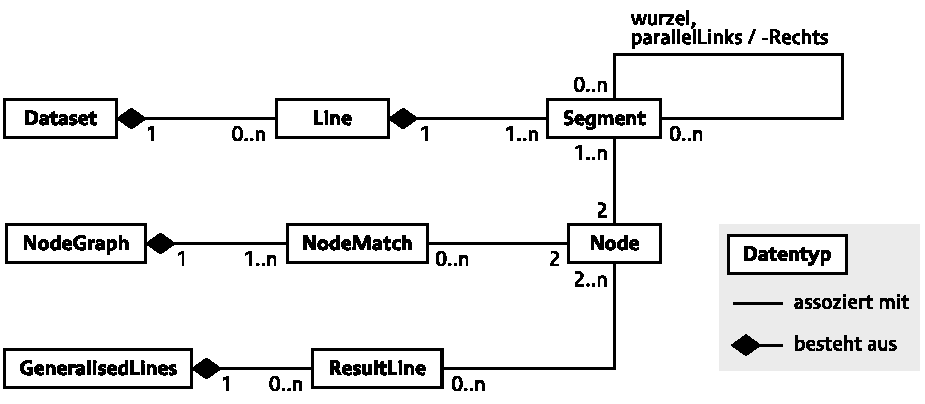
\includegraphics[scale=.69]{../appendices/data-model}
	\caption{Datenmodell}
	\label{fig:appx-data-model}
}

\onefigure{ht}{
	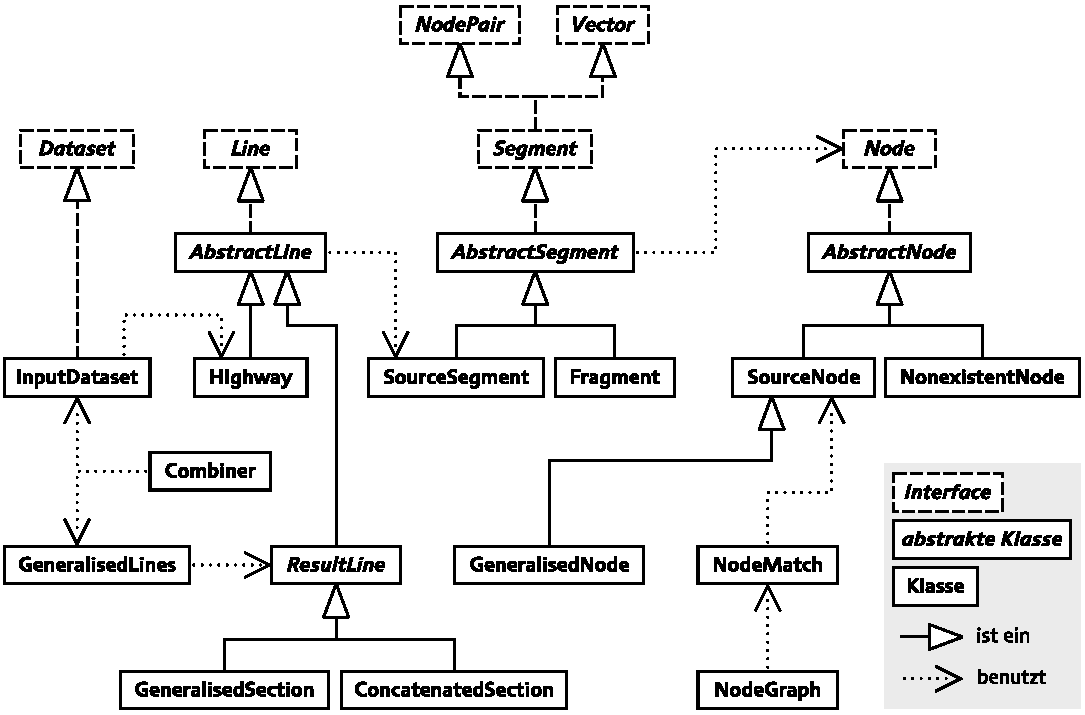
\includegraphics[scale=.69]{../appendices/class-structure}
	\caption
		[Klassenstrukturdiagramm für das Paket \code{comb}]
		{Klassenstrukturdiagramm für das Paket \code{comb} (aus Gründen der Übersichtlichkeit ist nur eine Auswahl der „benutzt“-Beziehungen dargestellt)}
	\label{fig:appx-class-structure}
}



\chapter{Anwendung auf ein Fernstraßennetz}
\label{appx:fullpage-examples-1}
% zu 6
% Beispiel für größeres Gebiet im Zusammenhang in kleinem Maßstab; evtl. unterschiedliche Regionen der Welt
% (Titel könnte sich noch ändern, vgl. E)

TBD



\chapter{Anwendung auf ein innerstädtisches Straßennetz}
\label{appx:fullpage-examples-2}
% zu 6
% Beispiel für größeres Gebiet im Zusammenhang in großem Maßstab; evtl. unterschiedliche Regionen der Welt
% (Titel könnte sich noch ändern, vgl. D)

TBD



\setcounter{chapter}{5}
\chapter{Beispiele für problematische Kreuzungssituationen}
\label{appx:junction-examples}
% zu 6

TBD\\
\\
(weitere Beispiele des Scheiterns an unterschiedlichen Kreuzungen; auch zeigen, wie \term{\_links} das Topologielückenproblem hierbei nicht lösen, sondern vergrößern)



%\chapter{Glossar}
%\chapter{Abkürzungsverzeichnis}
%\chapter{Software-Dokumentation}


% single-chapter commands
\end{document}
